\section{Introduction}
\label{sec:introduction}

Proponents of machine learning claim human
parity on tasks like reading comprehension~\cite{yu2018qanet}
and commonsense
inference~\cite{devlin2018BERT}. Despite these successes,
many evaluations neglect that computers solve natural language
processing \abr{nlp} tasks 
in a fundamentally different way than humans.  

Models can succeed without developing ``true'' language understanding,
instead learning superficial patterns from
crawled~\cite{chen2016thorough} or manually annotated
datasets~\cite{kaushik2018reading,gururangan2018annotation}.  Thus,
recent work stress tests models via adversarial evaluation:
elucidating a system's capabilities by exploiting its
weaknesses~\cite{jia2017adversarial,belinkov2019survey}.
Unfortunately, while adversarial evaluation reveals simplistic model
failures~\cite{ribeiro2018sear,mudrakarta2018understand}, exploring
more complex failure patterns requires human involvement (Figure~\ref{fig:flow_chart}):
automatically modifying natural language examples
without invalidating them is difficult. Hence, the diversity
of adversarial examples is often severely restricted.
	
\begin{figure*}[t]
\centering
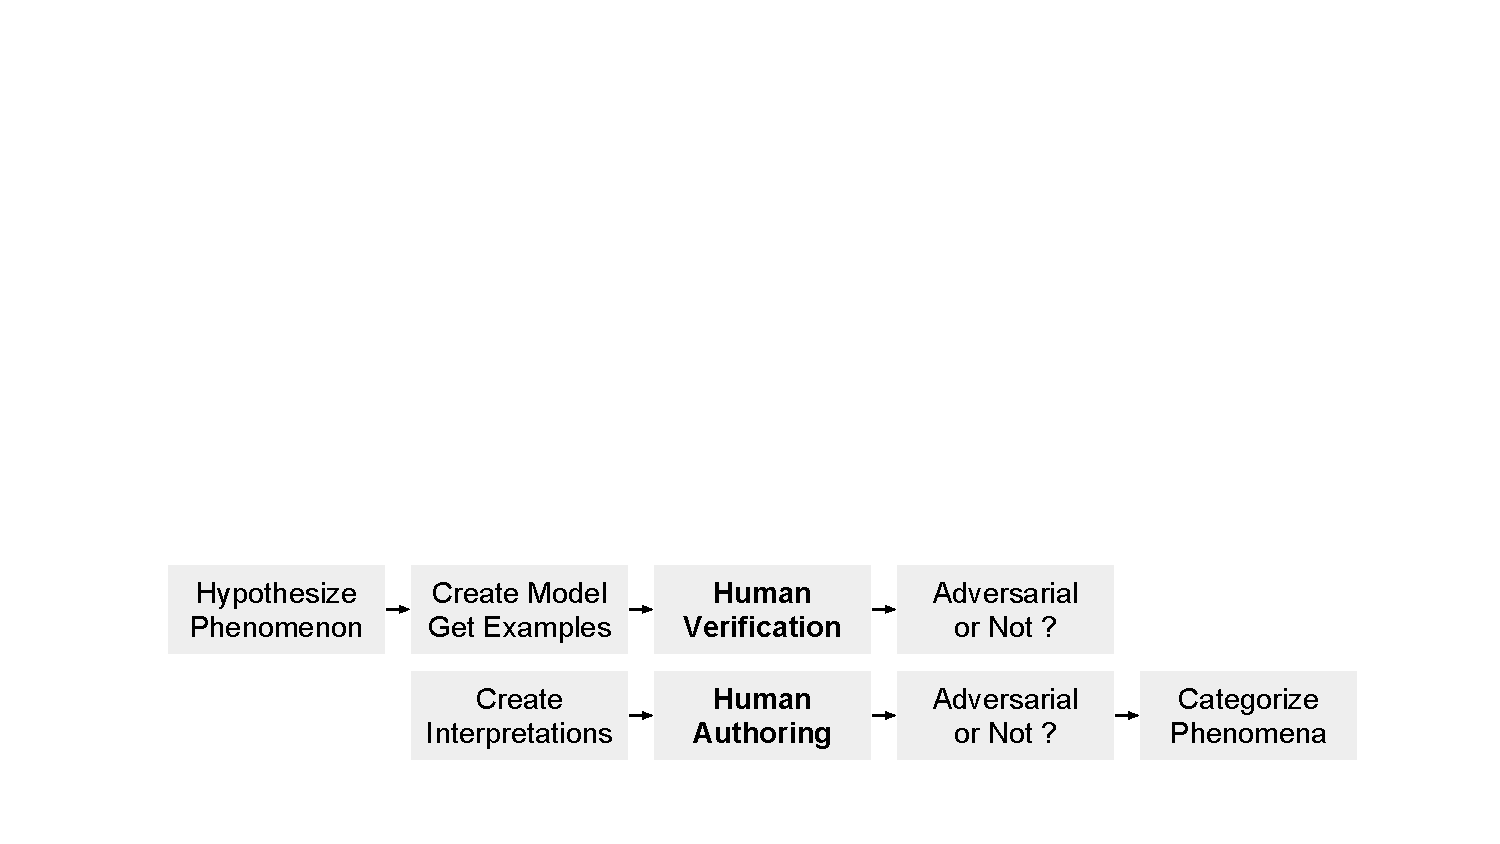
\includegraphics[width=0.8\linewidth, trim=0.0cm 0.3cm 0cm 0.2cm, clip]{flow_chart_horizontal}
\caption{Adversarial evaluation in \abr{nlp} typically focuses on a specific
  phenomenon (e.g., word replacements) and then generates the corresponding examples (top).
  Consequently, adversarial examples are limited to
  the diversity of what the underlying generative model or perturbation rule can produce and also require downstream
  human evaluation to ensure validity. Our setup (bottom) instead has
  human-authored examples, using human--computer collaboration to craft adversarial examples with greater diversity.}
\label{fig:flow_chart}
\end{figure*}

Instead, our human--computer hybrid approach uses human creativity to
generate adversarial examples.  A user interface presents model
interpretations and helps users craft model-breaking examples
(Section~\ref{sec:dataset}).  We apply this to a question answering
(\abr{qa}) task called \qb{}, where trivia enthusiasts---who write
questions for academic competitions---create diverse examples
that stump existing \abr{qa} models.

The \challenge{} test set is nonetheless as easy as
regular questions for humans (Section~\ref{sec:human}), but
the relative accuracy of strong \abr{qa} models drops as much as 40\%
(Section~\ref{sec:experiments}).
We also host live human vs. computer matches---where models typically defeat
top human teams---but observe spectacular model failures
on adversarial questions.

Analyzing the adversarial edits uncovers phenomena
that humans can solve but computers cannot
(Section~\ref{sec:limitations}), validating that our framework
uncovers creative, targeted adversarial edits (Section~\ref{sec:help}).
Our resulting adversarial dataset presents a fun, challenging,
and diverse resource for future \abr{qa} research: a system that masters
it will demonstrate more robust language understanding.